\begin{activity}{Warm-up: Two Bumps, One Line}


\begin{questions}
    \question{The mystery profile}
    Below is a gravity profile collected across an unknown structure.

    \begin{figure}[h]
        \centering
        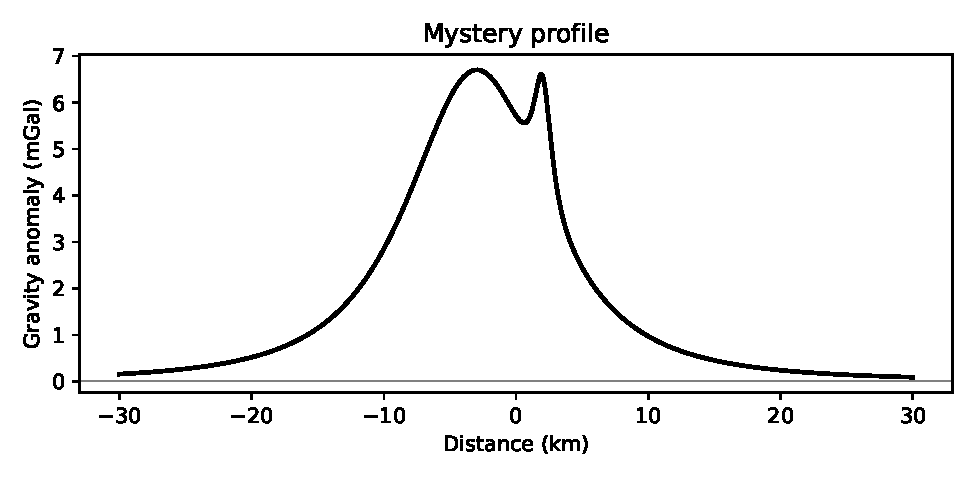
\includegraphics[width=0.75\textwidth]{figures/fig_mystery.pdf}
        \caption{Mystery gravity profile.}
    \end{figure}

    \begin{enumerate}[label=\roman*]
        \item Is this profile more consistent with a single buried source, or more than one? What in the shape of the curve makes you say so?
        \answerbox[2cm]

        \item If you think there could be more than one source, would you expect them to be at the same depth, or different depths? Why?
        \answerbox[2cm]

        \item Suppose the answer really is two sources at very different depths. Once they're added together into the single curve above, has the shallow source's signature been destroyed --- or is it still in there somewhere, just harder to see?
        \answerbox[2cm]
    \end{enumerate}
\end{questions}

\bigskip

\textit{Do not turn the page until your instructor asks you to.}

\newpage

\begin{questions}[resume]
    \question{The reveal}

    The mystery profile is the sum of two buried-sphere anomalies at different depths. On the left, the two components are shown separately; on the right, each component's \textbf{amplitude spectrum} --- the strength of each wavelength present in that signal.

    \begin{figure}[h]
        \centering
        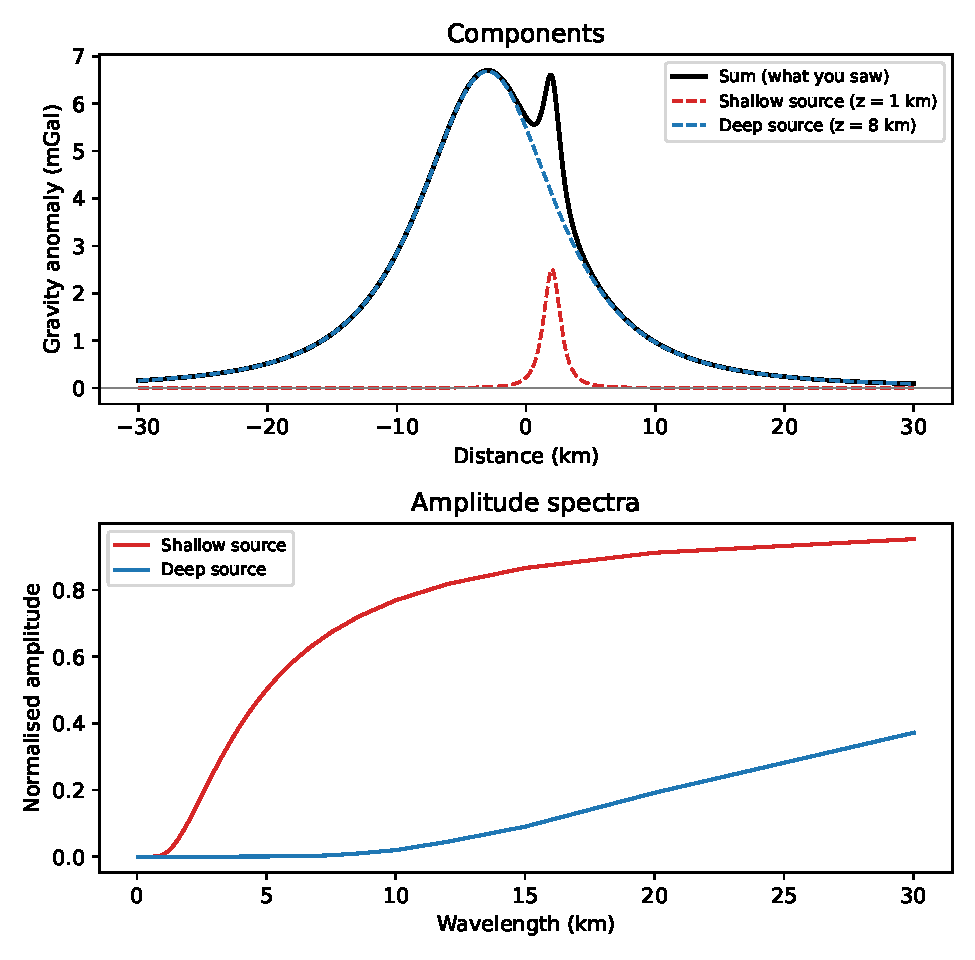
\includegraphics[width=0.75\textwidth]{figures/fig_reveal.pdf}
        \caption{(top) Revealed gravity field and (bottom) Fourier amplitudes for the individual bodies.}
    \end{figure}

    \begin{enumerate}[label=\roman*]
        \item Which source's spectrum is concentrated at short wavelengths, and which at long wavelengths? Does this match your intuition from Week 4 about width and depth?
        \answerbox[2cm]

        \item The two amplitude spectra barely overlap. What does that suggest about a strategy for separating a deep signal from a shallow one, \emph{without} ever looking at their depths directly?
        \answerbox[2cm]
    \end{enumerate}
\end{questions}

\bigskip

\textbf{Key Idea:} Depth behaves like a filter --- a deep source physically cannot produce short-wavelength anomalies, no matter how sharp the underlying body is. Keep this in mind today: you will meet it again, deliberately exploited, when we discuss isostatic filtering.

\end{activity}
